\documentclass[12pt,fleqn,a4paper,twoside]{mybook} %Final!!!

%\usepackage{microtype}
\usepackage[slovak]{babel}
\usepackage[utf8]{inputenc}
\usepackage[T1]{fontenc}
\usepackage[normalem]{ulem}
\usepackage{mathtools}  					
\usepackage{graphicx}
%\usepackage{subfig}
\usepackage{subfigure}
\usepackage{pdfpages}
\usepackage{enumerate}
\usepackage{etoolbox}                       %Problematic URL in reference
\apptocmd{\sloppy}{\hbadness 10000\relax}{}{}%Removes badness warnings
%This is to remove warnings resulting by otherwise OK URL's
\usepackage[hyphens]{url}
\usepackage{notes}
\usepackage{indentfirst}
\usepackage{makecell}
\renewcommand\theadfont{\bfseries\sffamily}
%\usepackage[demo]{graphicx}
\usepackage{upgreek}
\usepackage{multicol}
\usepackage{eurosym}
%This custom command defines how the literal menus look like.
\newcommand{\gui}[1]{{\emph{#1}}} %Gui commands, icon names, buttons
 % All code, functions, variables are typed like this
\newcommand{\code}[1]{{\lstinline[columns=fixed]{#1}}}

\newcommand{\angl}[1]{{\footnote{\emph{angl.}\ {#1}}}} %Shorthand english equivalent


\usepackage[inner=3.5cm,outer=2cm,top=25mm,bottom=25mm,paperwidth=210mm,paperheight=297mm,includehead]{geometry}

\usepackage{titlesec}
\titleformat{\chapter}[hang]{\normalfont\huge\bfseries}{\thechapter}{1em}{}


\DeclarePairedDelimiter{\diagpars}{(}{)}
\newcommand{\diag}{\operatorname{diag}\diagpars}

\let\oldhat\hat
\renewcommand{\vec}[1]{\boldsymbol{\mathbf{#1}}}
%\renewcommand{\hat}[1]{\oldhat{\boldsymbol{\mathbf{#1}}}}


\usepackage{amsthm}
\usepackage{etoolbox}% http://ctan.org/pkg/etoolbo
\theoremstyle{definition}
\newtheorem{exmp}{Pr\'{i}klad}[chapter]
\AtEndEnvironment{exmp}{\null\hfill\qedsymbol}

\usepackage{listings,color} 			    %To list Matlab code


\usepackage{xcolor}

\definecolor{Myblack}{RGB}{48, 55, 54}
\definecolor{Mybrown}{RGB}{15, 153, 117}
\definecolor{Mygreen}{RGB}{160, 82, 131}
\definecolor{Myyellow}{RGB}{208, 170, 91}
\definecolor{Myblue}{RGB}{4, 118, 249}

\lstset{language=C++,
	basicstyle=\ttfamily,
	keywordstyle=\color{Myblue}\ttfamily,
	stringstyle=\color{Myyellow}\ttfamily,
	commentstyle=\color{Mygreen}\ttfamily,
	numbers=none,
	breaklines=true,
	showspaces=false,
	showstringspaces=false
	backgroundcolor=\color{white}, % set backgroundcolor
	basicstyle=\footnotesize,% basic font setting
	morecomment=[l][\color{Mybrown}]{\#}
}

\renewcommand\lstlistingname{Zdrojový kód}
\renewcommand\lstlistlistingname{Zoznam zdrojového kódu}

\pagestyle{empty}

\begin{document}
%%%%%%% Zaciaatok %%%%%%%%
\includepdf[pages=-]{Title.pdf}
\includepdf[pages=-]{Blank.pdf}
\includepdf[pages=-]{RealTitle.pdf}
\includepdf[pages=-]{Blank.pdf}
\frontmatter
\includepdf[pages=-]{zadanie.pdf}
\includepdf[pages=-]{Blank.pdf}
 \null
\vfill
\noindent
\section*{Čestné prehlásenie}

Vyhlasujem, že predloženú záverečnú prácu som vypracoval samostatne pod vedením vedúceho záverečnej práce, s použitím odbornej literatúry a ďalších informačných zdrojov, ktoré sú citované v práci a uvedené v zozname použitej literatúry. Ako autor záverečnej práce ďalej prehlasujem, že som v súvislosti s jej vytvorením neporušil autorské práva tretích osôb.\\

\noindent Bratislava, 27. máj 2022 \hfill $\begin{array}{rl}
                                          &\text{..................................}\\
                                          &\text{Vlastnoručný podpis}\\
                                           \end{array}$
\cleardoublepage


	

 \null
\vfill
\noindent

V prvom rade by som sa chcel poďakovať vedúcej mojej bakalárskej práce, Ing. Mgr. Anne Vargovej, za výborne kávičky v kabinete, najlepšie meme obrázky v skupine ako aj za cenné rady a nekonečné opravy tejto práce. Ďalej chcem poďakovať aj Ing. Erikovi Mikulášovi, za pomoc pri tvorbe a kontrole (skoro)všetkých elektronických komponentov AeroShieldu, ako aj za pevné ruky pri spájkovaní. Ďakujem aj mojej partnerke Slávke, za to že každý deň trpezlivo počúvala moje nekonečné nadávky, sťažnosti ale aj radosti, pri tvorbe tejto práce. Zároveň sa chcem ospravedlniť spolužiakom, za stres ktorý mali z toho, keď som sa chválil 40. stranou práce, zatiaľ čo podaktorý ešte nepoznali tému ich BP.\\

\noindent Bratislava, 20. mája 2018 \hfill  Peter Tibenský
\cleardoublepage


	


 \noindent
\textbf{Názov práce:} AeroShield: Miniatúrny experimentálny modul aerokyvadla\\
\textbf{Kľúčové slová: } Arduino UNO, AutomationShield, PID, AeroShield, AeroPendulum \\
\textbf{Abstrakt: } Cielom bakalárskej práce je návrch experimentálneho modulu pre platformu Arduino. Tento modul má podobu externého shieldu, ktorý sa dá jednoducho pripojiť ku doskám Arduino a slúži na výučbu základov riadenia. Ich súčasťou je hardwareova a softwaerova časť. V rámci bakalárskej práce bol navrhnutý jeden modul s názvom AeorShield.   \\

\noindent
\textbf{Title:}AeroShield: Miniature experimental module of aeropendulum \\
\textbf{Keywords: }  Arduino UNO, AutomationShield, PID, AeroShield, AeroPendulum\\
\textbf{Abstract: } The aim of the bachelor's thesis is to design an experimental module for the Arduino platform. This module takes the form of an external shield that can be easily connected to Arduino boards and is used to teach the basics of control. Each module consist of hardware and a software part. As a part of this bachelor thesis, one module was designed, the AeroShield.
\cleardoublepage

%%%%%% \chapter*{Predhovor}
\thispagestyle{empty}

Myslel som si že ma táto téma bude baviť. Až pokial som si neuvedomil, že to nebude až také jednoduché... 

Už od malička ma fascinovala elektronika a všetko čo sa vedelo pohybovať a ja som to vedel riadiť. Volba tejto bakalárskej práce preto bola jasnou voľbou. 

\cleardoublepage

 %%%%%%
\tableofcontents
\thispagestyle{empty}
\cleardoublepage
\setcounter{page}{1}
% \phantomsection
\addcontentsline{toc}{chapter}{\listfigurename}
\listoffigures
\cleardoublepage
% \phantomsection
\addcontentsline{toc}{chapter}{\lstlistlistingname}
\lstlistoflistings
\newpage
%%%%%% Jednotlive kapitoly %%%%%%%%%
\pagestyle{plain}
\pagenumbering{arabic}
\setcounter{page}{1}

\mainmatter
\chapter*{Úvod}
\label{UVOD}
\addcontentsline{toc}{chapter}{Úvod}

%V úvode autor podrobnejšie ako v predhovore, pritom výstižne a krátko charakterizuje stav poznania alebo praxe v špecifickej oblasti, %ktorá je predmetom záverečnej práce. Autor presnejšie ako v predhovore vysvetlí ciele práce, jej zameranie, použité metódy a stručne %objasní vzťah práce k iným prácam podobného zamerania. V úvode netreba zachádzať hlbšie do teórie. Netreba podrobne opisovať metódy, %experimentálne výsledky, ani opakovať závery prípadne odporúčania.
%Úvod začína na novej  strane.


Cieľom tejto bakalárskej práce je návrh, výroba a naprogramovanie modernej učebnej pomôcky AeroShieldu (ďalej len „shield”), ktorý slúži na výuku základov teórie riadenia a elektrotechniky.

Učebné pomôcky sú nevyhnutnou, no často zanedbávanou súčasťou výuky. Študenti si vďaka nim môžu lepšie predstaviť a pochopiť problematiku daného učiva, keďže môže pracovať nie len s počítačovými modelmi sústavy, ale aj s jej fyzickou reprezentáciou. 
Avšak, takéto pomôcky bývajú častokrát príliš zložité na používanie a drahé \cite{Hor}. Z toho dôvodu, je ich použitie pri výučbe nepraktické.

Za cieľom sprístupnenia experimentálnych modulov širokej verejnosti bol založený projekt AutomationShield, ktorý ponúka pomerne jednoduché a cenovo dostupné experimentálne moduly ako open-source\footnote[1]{Open-source je zo všeobecného pohľadu akákoľvek informácia ktorá je dostupná verejnosti bez poplatku(s voľným prístupom), s ohľadom na fakt, že jej voľné šírenie zostane zachované.} študentské projekty.

Vhodnou platformou na implementáciu týchto modulov sú napríklad prototypizačné dosky Arduino ktoré sú taktiež open-source. Ich nízka cena a celosvetová popularita, spojená s obrovským množstvom návodov, informácii a pomôcok, vytvára ideálnu platformu pre začínajúcich, ako aj pokročilých, programátorov, elektrotechnikov alebo hobby nadšencov.

V bakalárskej práci je opísaný postup výroby a fungovania shieldu s dôrazom na zrozumiteľnosť jednotlivých aspektov aj čitateľom, ktorý o danej téme nie sú dokonale oboznámený. Na začiatku bakalárskej práce, v časti hardware, je opísaný základný princíp fungovania shieldu a následne jeho jednotlivé súčiastky. Pochopenie fungovania jednotlivých súčiastok shieldu je kritické pre správnu manipuláciu užívateľa s jeho jednotlivými časťami. Poslednú časť tvorí tvorba dosky plošných spojov pre shield v programe DipTrace.

V softvérovej časti sú bližšie predstavené jednotlivé charakteristické funkcie shieldu. Funkcie sú usporiadané do logických celkov pre ľahšiu prácu užívateľa s kódom.


\chapter{AeroShield}

Téma tejto bakalárskej práce vznikla ako pokračovanie, na už započatom projekte. Prvá verzia dosky a samotného kyvadla, vznikla ako záverečný projekt na predmet mikroprocesorová technika. Schému zapojenia hlavnej dosky, ako aj fotografiu zostavenej verzie, môžeme vidieť na obr.\ref{OBRAZOK 2.1.1}.


\begin{figure}[!tbh]
	\centering
	\includegraphics[width=80mm]{obr/oldshield.jpg}
	
	(a)
	\includegraphics[width=\linewidth]{obr/oldshieldscheme.png}
	(b)
	\caption{(a) Prvá verzia AeroShieldu. (b) Schéma zapojenia prvej verzie AeroShieldu.}
	\label{OBRAZOK 2.1.1}
\end{figure}

\vspace{3cm}

Prvá verzia dosky mala niekoľko nedostatkov, vďaka ktorým bola prakticky nepoužiteľná. Hlavnými nedostatkami boli:

\begin{itemize}
	\item neprepojenie pinov komunikácie I2C tj. piny SDA a SCL senzoru hall efektu, ktorý slúži na meranie uhlu natočenia kyvadla,
	\item nesprávne zapojenie mosfetu PMW45EN, ktorý ovláda PWM signál idúci do akčného člena,
	\item nesprávne umiestnená ochranná dióda na konektoroch akčného člena,
	\item nesprávne zapojený obvod s čipom INA169, ktorý slúži na meranie prúdu,
	\item neprepojenie nulového konektora shieldu s nulovým konektorom arduina.
\end{itemize}

Základom tejto bakalárskej práce teda bolo, pochopiť jednotlivé časti zapojenia, analyzovať chyby a ich následná oprava. V rámci školského projektu bola vytvorená hlavná doska, na ktorej sa nachádza väčšina elektroniky a menšia, vedľajšia doska, ktorá slúži na fungovanie senzoru hall efektu. Táto doska fungovala bezproblémovo a teda nebolo potrebné nijakým spôsobom meniť jej schému zapojenia, viditeľnú na obr.\ref{OBRAZOK 2.1.2}.a. Tejto menšej doske sa budeme bližšie venovať v časti \ref{PCBcka}, no jej podoba je viditeľná na obr.\ref{OBRAZOK 2.1.2}.b.

\begin{figure}[!tbh]
	\hfill
	\subfigure[Schéma zapojenia externej dosky.]{\includegraphics[width=9cm]{obr/as5600.png}}
	\hfill
	\subfigure[Doska slúžiaca na fungovanie senzoru hall efektu.]{\includegraphics[width=5cm]{obr/fotoBreak.png}}
	\hfill
	\caption{meranie uhla kyvadla}\label{OBRAZOK 2.1.2}
\end{figure}



\newpage
\section{Hardware}
\subsection{Popis súčiastok}

V tejto časti sa bližšie pozrieme na jednotlivé nevyhnutné súčasti zapojenia AeroShieldu. Konkrétne sa jedná o tieto prvky:
\begin{multicols}{2}
	\begin{itemize}
		\item napájanie
		\item ovládanie akčného člena
		\item meranie uhla natočenia kyvadla
		\item meranie prúdu
	\end{itemize}
\end{multicols}


\subsubsection{Znižovací menič}
\label{nap}

Na správne napájanie akčného člena, motorčeka, potrebujeme napätie v rozmedzí 0-3,7V. Na shield je však privádzané, pomocou koaxiálneho napájacieho konektora, napätie 12V, ktoré by motor v priebehu chvíle zničilo. Na zníženie napätia preto použijeme znižovací menič tzv. buck converter. 

Hlavnou časťou konvertora je čip TPS56339 od výrobcu Texas Instruments obr.\ref{OBRAZOK 2.1}.b. Znižovanie napätia funguje za pomoci dvoch integrovaných N-kanálových 70-m$\Omega$ a 35-m$\Omega$ high-side mosfetov\footnote[4]{N-kanálový mosfet je typ mosfetu, v ktorom tok prúdu nastáva kvôli pohybujúcim sa, záporne nabitým elektrónom. $"High-side"$ znamená, že prúd prechádza z napájania, cez mosfet, do záťaže a potom do zeme.}, v spolupráci s ďalšími komponentami. Celkový prevádzkový prúd zariadenia je približne 98$\upmu$A, keď funguje bez spínania a bez záťaže. Keď je zariadenie vypnuté, napájací prúd je približne 3$\upmu$A a zariadenie umožňuje nepretržitý výstupný prúd do 3 A\cite{buckobr}.

\begin{figure}[!tbh]
	\hfill
	\subfigure[Schéma zapojenia znižovacieho meniča.]{\includegraphics[width=9cm]{obr/schemaBuck.png}}
	\hfill
	\subfigure[{čip TPS56339.\cite{buckobr}}]{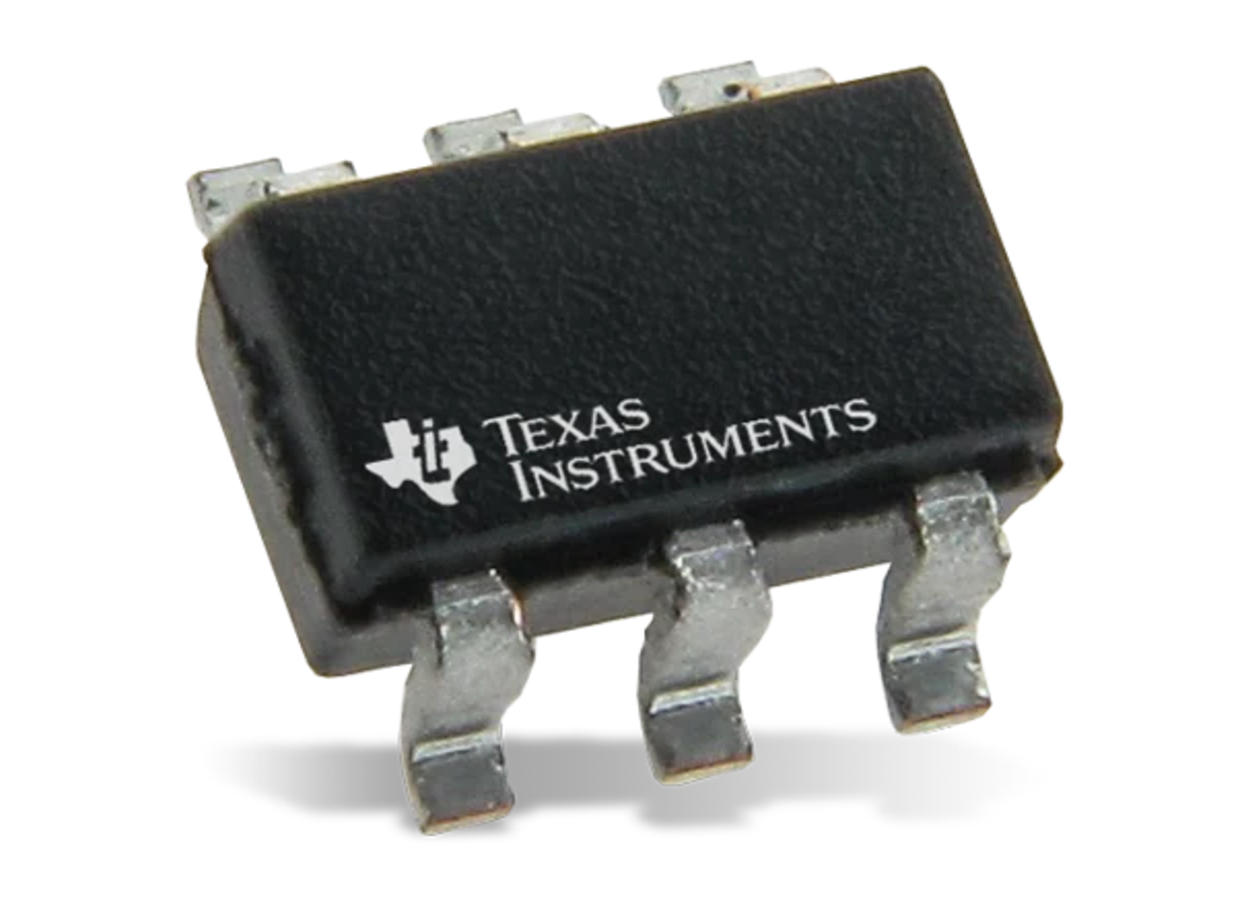
\includegraphics[width=5cm]{obr/cip.eps}}
	\hfill
	\caption{buck converter}\label{OBRAZOK 2.1}
\end{figure}

Na čip je privádzané napätie 12V ktoré sa pomocou zapojenia viditeľného na schéme obr.\ref{OBRAZOK 2.1}.a, znižuje na napätie 3,7V. Napájanie motora musí byť realizované externe pomocou koaxiálneho napájacieho konektora, z dôvodu vysokého prúdu odoberaného motorom počas silného zaťaženia. Rovnaký konektor sa síce nachádza aj na doske Arduino UNO a pomocou VIN pinu sa z neho dajú napájať napätím 12V aj iné zariadenia, avšak tento pin je napojený na diódu, obmedzujúcu prúd na 1A\cite{ampere}\cite{ampere2}.

\subsubsection{akčný člen}
\label{akcclen}

Ako akčný člen AeroShieldu je použitý 7mm, 3,7V motorček na jednosmerný prúd bez jadra, používaný hlavne pre pohon dronov. “Coreless motor“, alebo motor bez jadra, je motor s cievkou navinutou samou na sebe a nie na železe\cite{coreless}. Takéto jadro ale samé o sebe nie je veľmi pevné a nedrží dobre tvar, preto sa častokrát zalieva epoxidom. Stator je vyrobený z magnetov na báze vzácnych zemín, ako je neodým alebo SmCo(samárium-kobalt), ktoré sa nachádzajú vo vnútri bezjadrového rotora.

Takýto motor ponúka mnoho výhod oproti motoru so železným jadrom. Tým že jadro v sebe nemá železo, výrazne sa znižuje hmotnosť a tým aj zotrvačnosť rotora, čo je dôležité pre naše použitie, kedy potrebujeme dosahovať vysokú akceleráciu a rýchle spomalenie rotora. Ďalšou výhodou je fakt, že nedochádza k stratám na železe a tým pádom sa účinnosť takýchto motorov blíži až ku 90\%\cite{5545147}. Motor, resp. otáčky motora sú riadené pomocou impulzovej šírkovej modulácie(PWM) a tieto impulzy do motoru prechádzajú cez N-kanálový mosfet PMV45EN2 od výrobcu Nexperia\cite{pmv}.


\begin{figure}[!tbh]
	\hfill
	\subfigure[Schéma zapojenia motorčeka.]{\includegraphics[width=7cm]{obr/MotorScheme.png}}
	\hfill
	\subfigure[{Akčný člen sústavy.\cite{corelessMotor}}]{\includegraphics[width=7cm]{obr/coreless.jpg}}
	\hfill
	\caption{Zapojenie akčného člena a typ motorčeka}\label{OBRAZOK 2.3}
\end{figure}


\subsubsection{meranie prúdu}
\label{merprud}

Z dôvodu merania prúdu odoberaného motorom, bol do schémy pridaný monitor prúdu, takzvaný "current shunt monitor". V AeroShielde je použitý snímač INA169NA/250 od výrobcu Texas Instruments obr.\ref{OBRAZOK 2.3.2}.b.

INA169 funguje na základe zaznamenávania zmien napätia na stranách shunt rezistora obr.\ref{OBRAZOK 2.3.2}.a. Na základe nameraného úbytku napätia, vysiela senzor podľa nami zvoleného stupňa zosilnenia, prúd ktorý je ďalej pomocou rezistoru $R_{l}$ premenený na napätie s maximálnou hodnotou $V_{OUTMAX} = V_{IN-} - 0.5V $.

Prúd $I_{s}$ odoberaný motorom, vypočítame pomocou vzorca $I_{s} = \dfrac{V_{OUT}\: x \: 1k\Omega}{R_{s} \: x \: R_{l}} $ kde $V_{OUT}$ je napätie namerané na výstupe, 1k$\Omega$ je konštanta vnútorných odporov senzoru, $R_{s}$ je hodnota shunt rezistora v $\Omega$ a $R_{l}$ je hodnota rezistora na výstupe, taktiež v $\Omega$\cite{INA}.

\begin{figure}[!tbh]
	\hfill
	\subfigure[Schéma zapojenia snímača prúdu.]{\includegraphics[width=9cm]{obr/INAschema.png}}
	\hfill
	\subfigure[{Senzor INA169NA/250\cite{INAobr}}]{\includegraphics[width=6cm]{obr/ina.png}}
	\hfill
	\caption{meranie prúdu}\label{OBRAZOK 2.3.2}
\end{figure}


\label{Hall}
\pagebreak

\subsubsection{meranie uhla kyvadla}
\label{meruhl}

Na správne fungovanie AeroShieldu je dôležité vedieť s vysokou presnosťou merať uhol naklonenia kyvadla. Na tento účel sme si zvolili meranie uhlu bez kontaktnou formou, pomocou snímača hall efektu. Hall efekt vieme opísať ako vznik priečneho elektrického poľa v pevnom materiáli, keď ním preteká elektrický prúd a tento materiál je umiestnený v magnetickom poli, ktoré je kolmé na prúd\cite{Hall}. Toto elektrické pole resp. vznik elektrického potenciálu vieme detegovať a na základe jeho zmeny vieme určiť rotáciu kyvadla. V kyvadle je na konci horizontálneho ramena umiestnený špeciálny magnet kruhového tvaru, ktorý je polarizovaný naprieč prierezom magnetu.

Ako senzor na meranie hall efektu je použitý AS5600 od výrobcu OSRAM obr.\ref{OBRAZOK 2.2}.b. Signály prichádzajúce zo snímača sa najprv zosilnia, následne sú filtrované a prechádzajú konverziou pomocou analógovo-digitálneho prevodníka(ADC). Snímaná je aj intenzita magnetického poľa, ktorá sa ďalej používa na
automatické riadenie zosilnenia(AGC), ktoré slúži na kompenzáciu teploty priestoru a magnetu a veľkosti magnetického poľa.

Na výber sú dva typy výstupu a to analógový výstup alebo digitálny výstup s kódovaním PWM. Senzor má taktiež možnosti interného programovania pomocou rozhrania I2C.
V našom prípade používame 12-bitový analógový výstup s rozlíšením 0°5'16". Toto rozlíšenie nám umožňuje s vysokou presnosťou kontrolovať naklonenie kyvadla a na základe získaných informácii ovplyvňovať fungovanie akčného členu sústavy. Schéma zapojenia čipu na meranie uhlu môžeme vidieť na obr.\ref{OBRAZOK 2.2}.a.



\begin{figure}[!tbh]
	\hfill
	\subfigure[Schéma zapojenia čipu na meranie uhlu.]{\includegraphics[width=10cm]{obr/as5600.png}}
	\hfill
	\subfigure[{čip AS5600\cite{As5600obr}}]{\includegraphics[width=4cm]{obr/hall.jpg}}
	\hfill
	\caption{meranie uhla kyvadla}\label{OBRAZOK 2.2}
\end{figure}

\newpage


\subsection{Schéma zapojenia}

Všetky schémy zapojenia boli tvorené v bezplatnej verzii programu DipTrace. DipTrace slúži ako prostredie na tvorbu elektrotechnických schém, potrebných pre výrobu dosiek plošných spojov, ako aj pre účely prehľadnosti zapojenia komponentov na týchto doskách. Program v sebe zahŕňa časť pre tvorbu samotných komponentov, pokiaľ sa tieto už nenachádzajú v niektorej z knižníc programu, časť kde sa tvoria schémy zapojenia a časť na tvorbu dosiek plošných spojov.

Nie všetky komponenty potrebné na tvorbu AeroShieldu boli zahrnuté v knižniciach DipTracu, avšak tieto komponenty sa nachádzali na stiahnutie na stránkach výrobcov odkiaľ boli importované do novej knižnice, slúžiacej na účely tvorby schémy AeroShieldu. Do programu bola taktiež vložená knižnica AutomationShieldu ktorá má v sebe najčastejšie používané komponenty. Pri tvorbe schémy zapojenia sa najskôr všetky potrebné komponenty umiestnia na štvorčekovú plochu a približne sa určí ích poloha. Jednotlivé komponenty majú podobu elektrotechnických značiek a každý komponent má ku sebe priradené reálne vlastnosti daného dielu(veľkosť, zapojenie, dĺžka pinov a iné).

Polohu volíme takú, aby schéma bola čo najprehľadnejšia a komponenty ktoré sú medzi sebou prepojené, boli čo najbližšie pri sebe. Akonáhle máme všetky komponenty uložené začneme s ich postupným prepájaním. Pri zapájaní jednotlivých komponentov sa riadime katalógovými listami jednotlivých komponentov, v ktorých býva zväčša aj návrh ich zapojenia.

Veľmi dobrou vlastnosťou programu DipTrace je možnosť zafarbovania jednotlivých elektrických spojení, rozličnými farbami a názvami. Tento fakt nám veľmi uľahčuje na prvý pohľad rozoznať napríklad elektrické spojenia zeme- 0V zelená, fázové spojenia- 3,3V červená obr.\ref{OBRAZOK 2.3.5}. Na schéme zapojenia môžeme vidieť všetky komponenty, potrebné na správne fungovanie AeroShieldu. Názvy komponentov sú uvádzané základnými značkami
\begin{multicols}{3}
	\begin{itemize}
		\item R- Rezistor
		\item C- Kapacitor
		\item J- Konektor
		\item U- Mikročip
		\item L- Cievka
		\item D- Dióda
		\item M- Motor
	\end{itemize}
\end{multicols}


\begin{figure}[!tbh]
	\includegraphics[width=\textwidth]{obr/aeroSchema.png}
	\caption{Schéma zapojenia AeroShieldu}\label{OBRAZOK 2.3.5}
\end{figure}

\subsection{Doska plošných spojov}
\label{PCBcka}

Po návrhu a kontrole schém zapojenia sa schémy ďalej spracovávajú do podoby dosky plošných spojov. Schémy exportujeme do programu DipTrace PCB v ktorom máme následne niekoľko možností postupu. Jednotlivé komponenty sa nám už zobrazujú v reálnej podobe, takže vidíme ich veľkosť a rozmiestnenie pinov na spájkovanie. Dosky plošných spojov majú niekoľko nevýhod, ale aj výhod oproti ponúkaným alternatívam\cite{dosky}. 

Výhodou je fakt, že vodivé spojenia medzi jednotlivými súčiastkami zapojenia, sú realizované vrstvou medi ktorá je ukrytá pod ochrannými vrstvami povrchu dosky, na rozdiel od typických káblových spojení. Káble majú niekoľko nedostatkov ako to že sa vedia ľahko vypojiť, ľahko dochádza k ich porušeniu a v neposlednom rade, nepôsobia veľmi esteticky. V prípade nesprávneho prepojenia pinov má jednoznačnú výhodu spoj realizovaný káblami, keďže pri doskách plošných spojov sa s už hotovými cestami manipuluje obtiažne. Ďalšou výhodou dosiek plošných spojov je skutočnosť, že sú veľmi odolné a kompaktné. Tým že vodivé cesty môžu mať veľmi malé rozmery, ovplyvňujúcim faktorom veľkosti dosky plošných spojov je samotná veľkosť jej komponentov. 

Po prenesení schém do DipTrace PCB, sú jednotlivé komponenty rozhádzané a nemajú žiadne logické rozloženie. Program ponúka možnosť automatického zoradenia komponentov na vyhradenej ploche, avšak táto funkcia komponenty uložila nie podľa našich potrieb a teda, využili sme možnosť manuálneho umiestnenia jednotlivých komponentov. Pri pohybovaní jednotlivými komponentami môžeme vidieť čiary, ktoré symbolizujú prepojenia s ostatnými komponentami a vďaka tomu vieme komponenty logicky poukladať.

\begin{figure}[!tbh]
	\hfill
	\subfigure[Vrchná strana breakout boardu]{\includegraphics[width=7cm]{obr/breakoutTOP.png}}
	\hfill
	\subfigure[Spodná strana breakout boardu]{\includegraphics[width=7cm]{obr/breakoutbottom.png}}
	\hfill
	\caption{Vedľajšia doska AeroShieldu- breakout board}\label{OBRAZOK 2.6}
\end{figure}

Po zvolení optimálneho rozmiestnenia komponentov treba jednotlivé piny poprepájať vodivými cestami, ktoré nám nahrádzajú funkciu káblov. Máme možnosť zvoliť automatické rozmiestnenie ciest alebo ich manuálnu tvorbu. V našom prípade sme zvolili manuálnu tvorbu ciest, pretože ich vieme čo najlepšie optimalizovať. Ako je viditeľné aj na obr.\ref{OBRAZOK 2.4}.a, nie všetky cesty majú rovnakú šírku. Je to z toho titulu že niektorými cestami prúdi vyšší prúd a to až do 1A. V zásade sa používa pravidlo, čím vyšší prú preteká vodičom, tým väčšiu plochu prierezu by mal mať. Prúdy pretekajúce vodičmi tieto vodiče zahrievajú a pokiaľ je toto zahrievanie nadmerné, môže dôjsť k poškodeniu vodiča.  

Tvorba ciest má niekoľko pravidiel, avšak najdôležitejšie z nich je že jednotlivé cesty ktoré v schéme zapojenia nie sú prepojené, sa nemôžu križovať inak dôjde k ich vzájomnému vyskratovaniu. Z toho dôvodu treba niekedy cestu priviesť na druhú stranu dosky plošných spojov kde v jej pokračovaní neprekáža iná cesta. Na tento účel sa používajú vodivé diery, takzvané via, spájajúce obe strany dosky.

Pri výroby dosky sa taktiež myslelo na montáž držiaku kyvadla, pre ktoré boli vytvorené 4 diery na jeho následné prichytenie pomocou skrutiek. Finálna verzia hlavnej dosky je na obr.\ref{OBRAZOK 2.4}. Zhotovená bola aj menšia doska tzv. breakout board, slúžiaca na meranie uhlu kyvadla, ktorá je na obr.\ref{OBRAZOK 2.6}.



\begin{figure}
	\centering
	\includegraphics[width=8cm]{obr/AeroShieldTOP.png}
	
	(a)
	
	\includegraphics[width=8.5cm]{obr/AeroShieldBOTTOM.png}
	
	(b)
	
	\caption{(a) Vrchná strana AeroShieldu (b) Spodná strana AeroShieldu}
	\label{OBRAZOK 2.4}
\end{figure}



Po finálnej kontrole zapojenia komponentov na doske plošných spojov môžeme tieto dosky uložiť do formátu gerber. Súbory typu gerber v sebe ukladajú presné zloženie finálnej dosky plošných spojov a to po jej jednotlivých vrstvách. Nachádza sa tu teda vrstva zobrazujúca vodivé cesty, vrstva pre konektory via, vrstva pre farebné popisy a mnoho ďalších. Pri tvorbe súboru máme veľa možností aké parametre jednotlivých vrstiev chceme zvoliť. Môžeme meniť hrúbky jednotlivých vrstiev, veľkostí dier a priestoru okolo dier, veľkosti konektorov via a iné. Gerber súbor ďalej posielame výrobcovi PCB dosiek kde si môžeme zvoliť ďalšie parametre dosky, ako jej farbu, možnosti spájkovacích doštičiek, dokonca nám môže výrobca poslať už naspájkovanú dosku, ktorá je tak hneď pripravená na použitie. Podobu finálnej dosky AeroShieldu môžeme vidieť na obr.\ref{OBRAZOK 2.7}.a a dosky breakout boardu na obr.\ref{OBRAZOK 2.7}.b.


\begin{figure}
	\hfill
	\subfigure[Hlavná doska AeroShieldu]{\includegraphics[width=9cm]{obr/AeroShield.jpg}}
	\hfill
	\subfigure[Vedľajšia doska AeroShieldu]{\includegraphics[width=6cm]{obr/fotoBreak.png}}
	\hfill
	\caption{Dosky plošných spojov AeroShieldu}\label{OBRAZOK 2.7}
\end{figure}

\subsection{Model držiaku kyvadla}

Tu ešte poviem čo to a designovaní držiaku pendulum

\subsection{Cenová kalkulácia AeroShieldu}

Hlavnou podmienku pri tvorbe AeroShieldu, bola jeho funkcionalita, no zároveň nízka cena. Za účelom predstavy cenovej relácie jedného kusu AeroShieldu, bola zostavená tabuľka\ref{Cenova kalkulacia} s použitými komponentami, ich počtom a reálnou kúpnou cenou v eurách(spolu s DPH). Pri komponentoch ako sú rezistory a kapacitory, bola cena určená ako priemerná hodnota týchto komponentov, keďže pri kúpe zopár kusov(1-20) je ich cena rádovo vyššia, ako cena pri nákupoch viacero kusov. 

\begin{table}[!ht]
	\begin{tabular}{p{0.25\textwidth} p{0.43\textwidth} p{0.05\textwidth} p{0.07\textwidth} p{0.07\textwidth}}
		\hline
		\multicolumn{1}{|l}{\textbf{Názov}} & \textbf{Popis}                                     & \multicolumn{1}{l}{\textbf{Ks.}} & \multicolumn{1}{l}{\textbf{Cena}} & \multicolumn{1}{l|}{\textbf{Spolu}} \\ \hline
		Kapacitor                           & SMD, sot23                                         & 6                                  & 0,6                                      & 3,6                                        \\
		Dióda                               & 1N400IG                                            & 1                                  & 0,1                                      & 0,1                                        \\
		FFC konektor                        & FFC 4pin                                           & 2                                  & 0,2                                      & 0,4                                        \\
		Cievka                              & IND1210                                            & 1                                  & 0,2                                      & 0,2                                        \\
		Konektor DC motora                  & JST-XH 2,54                                        & 1                                  & 0,4                                      & 0,4                                        \\
		Motor                               & Howellp 7x20mm Motor                               & 1                                  & 2,1                                      & 2,1                                        \\
		Potenciometer                       & CA14                                               & 1                                  & 0,45                                     & 0,45                                       \\
		Mosfet                              & pmv45en2                                           & 1                                  & 0,04                                     & 0,04                                       \\
		Rezistor                            & SMD, sot23                                         & 9                                  & 0,4                                      & 3,6                                        \\
		Buck converter                      & TPS56339                                           & 1                                  & 2,78                                     & 2,78                                       \\
		Shunt monitor                       & INA169/NA                                          & 1                                  & 0,98                                     & 0,98                                       \\
		Hall senzor                         & AS5600                                             & 1                                  & 1,48                                     & 1,48                                       \\
		3D komponenty                       & model kyvadla a spojovacie prvky                   & 4                                  & 2,2                                      & 2,2                                        \\
		Gulôčkové ložiská                   & BB-694-B180-30-ES IGUS                             & 2                                  & 2,75                                     & 5,5                                        \\
		Prepájacie káble FFC                & akékoľvek 4 pin, dĺžka min 15cm                    & 1                                  & 0,52                                     & 0,52                                       \\
		Prepajací kábel motor               & akékoľvek, dĺžka min 35cm                          & 1                                  & 0,3                                      & 0,3                                        \\
		Šróby                               & 4x M3x40 4x M4x15                                  & 8                                  & 0,25                                     & 2                                          \\
		Karbónové trubičky                  & 1x kruhový prierez 10cm, 1x štvorcový prierez 10cm & 2                                  & 1,9                                      & 3,8                                        \\
		PCB shield                          & Výroba JLCPCB                                      & 1                                  & 0,35                                     & 0,35                                       \\
		PCB brakout                         & Výroba JLCPCB                                      & 1                                  & 0,35                                     & 0,35                                       \\
		Matice                              & M4                                                 & 4                                  & 0,2                                      & 0,8                                        \\ \hline
		\multicolumn{1}{|l}{}               &                                                    & \multicolumn{1}{l}{}               & \textbf{Spolu}                           & \multicolumn{1}{c|}{\textbf{31,95}}        \\ \hline
	\end{tabular}
\caption{Cenová kalkulácia AeroShieldu.}
\label{Cenova kalkulacia}
\end{table}
\section{Software}

Programovacie rozhranie pre platformy arduino sa nazýva Arduino IDE\footnote[5]{Arduino Integrated Development Environment.} a využíva programovací jazyk C++ resp. jeho podobu, s pridanými špecializovanými príkazmi a funkciami priamo pre arduino IDE. Príkazy sú na prvý pohľad zrozumiteľnejšie ako ich skompilovaná\footnote[6]{Kompilácia je preklad zdrojového kódu do podoby ktorú vie procesor prečítať a spracovať.} podoba v jazyku C++, no funkcie resp. schopnosti príkazu sú rovnaké. Preto je arduino vhodným prostriedkom na programovanie ako pre začiatočníkov, tak aj pre skúsenejších programátorov. 

Pri tvorbe programovej časti AeroShieldu je dôležité uvedomiť si fakt že doska vzniká v rámci projektu AutomationShield. Tým že je tento projekt opensource, ktokoľvek môže kód upravovať a vylepšovať, je preto dôležité aby funkcie navádzali používateľov na ich správne použitie a aby boli čo najviac prehľadné. Z tohoto dôvodu bola vytvorená knižnica AutomationShield ktorá v sebe zahŕňa najviac používané funkcie. Predstavme si situáciu kedy v programe ktorý píšeme potrebujeme premenu jednotiek z metrov na centimetre. Pokiaľ takúto funkciu potrebujeme použiť v kóde jeden krát, môžeme túto funkciu napísať priamo do kódu. Avšak pokiaľ túto funkciu využívame častejšie, dáva zmysel uložiť ju mimo kód a následne túto funkciu zavolať naspäť v prípade jej potreby. Sprehľadňuje sa tak vzniknutý kód a znižuje sa možnosť chýb vďaka monotónnym kopírovaniam tej istej funkcie. 

Takúto možnosť externých preddefinovaných funkcií prístupných na zavolanie ponúka objektovo orientované programovanie(OOP) v jazyku C++. Zvyčajne sa vytvárajú dva súbory resp. knižnice, z ktorých jedna sa nazýva "header" alebo hlavička s koncovkou .h a druhá, "source" alebo zdrojový dokument s koncovkou .cpp. Header slúži ako akýsi navádzač a sklad pre premenné a funkcie, ktorý následne komunikuje so source dokumentom v ktorom sú uložené samotné funkcie. 

\subsection{Header}

Header súbor má niekoľko náležitostí ktoré obsahuje. Vytvárame v ňom "class" alebo triedu ktorá v sebe zahŕňa funkcie a premenné ktoré sa nazývajú "objects" alebo objekty. Class teda obsahuje podmnožinu objectov ktoré vieme prepájať a spájať vo väčšie celky, vďaka čomu vieme dosiahnuť veľmi komplexné funkcie. Tieto funkcie a premenné môžu byť buď "public" teda verejné a prístupné aj mimo súbor alebo "privat" teda súkromné ktoré su prístupné len v knižniciach header a source. Deklarácia takejto triedy vyzerá nasledovne: 


\begin{lstlisting}
	class AeroShield{		// Deklaracia triedy
		public :		// Verejna cast
		void FirstObject();	// Deklaracia funkcie
		
		private :		// Sukromna cast
		float FirstVariable;	// Deklaracia premennej
	};				// Koniec triedy
\end{lstlisting}
\newpage

V našom prípade nám postačuje jedna trieda ktorá sa nazýva AeroShield a má v sebe jednu funkciu s názvom FirstObject() v časti public a jednu premennú FirstVariable typu float v časti pivate. Rozdelenie na public a privat má zmysel hlavne v prípade ak chceme mať zadefinované isté premenné, pri ktorých nechceme aby sa dala externe zmeniť ich hodnota alebo typ. V prípade privat, takáto zmena nie je možná, jediná možnosť ako premennú zmeniť, je jej ručné prepísanie v súbore. V časti private deklarujeme funkcie ktoré následne využívame v rámci triedy a slúžia ako pomocné funkcie pri tvorbe komplexnejších častí kódu. V časti public sú funkcie viditeľné a schopné interagovať s inými triedami ako aj s inými knižnicami. 



\chapter{Didaktické príklady}
\label{Didaktické príklady}

Pre AeroShield bolo v prostredí Arduino IDE, MATLAB a Simulink vytvorených niekoľko vzorových programov, ktoré demonštrujú všetky jeho funkcie. Programy sú rozdelené do dvoch veľkých skupín, konkrétne programy v otvorenej slučke bez spätnej väzby a programy v uzavretej slučke so spätnou väzbou. 

Ich rozdiel spočíva v tom, že pri riadení bez spätnej väzby, hovoríme o ovládaní systému, kedy sa snažíme dosiahnuť žiadané hodnoty výstupov bez spätnej informácie o vykonaní procesu, alebo o jeho hodnote. V prípade riadenia so spätnou väzbou sa jedná o reguláciu. Pri regulácii sa kontroluje bezprostredný účinok riadenia, ktorý sa porovnáva so žiadanou hodnotou výstupu a na vyrovnanie ich vzájomnej chyby, sa okamžite vykonáva zásah do vstupných veličín. 

\section{Programy v otvorenej slučke, bez spätnej väzby}
\subsection{Arduino IDE}
\label{bezspatnej}

Ako prvý príklad si ukážeme program s názvom \verb|AeroShield_OpenLoop.ino| napísaný v prostredí Arduino IDE. Hlavnou ideou tohoto programu je jednoduché ovládanie otáčok motorčeka, pomocou potenciometra. Na začiatku programu inicializujeme hlavnú knižnicu AeroShieldu pomocou príkazu \verb|#include "AeroShield.h"|. Následne deklarujeme premenné, ktorých hodnoty budú vypisované na sériový monitor. 

\begin{lstlisting}[caption={AeroShield open loop dekleracia.},captionpos=b]
	float startangle=0;           //  Premenna pre nulovy uhol
	float lastangle=0;            //  Premenna pre maximalny uhol 
	float pendulumAngle;          //  Uhol natocenia kyvadla
	float referencePercent;       //  Hodnota potenciometra
	float CurrentMean;	      //  Hodnota prudu odoberaneho motorom 
\end{lstlisting}

V časti \verb|setup()| ako prvé prebehne nastavenie rýchlosti sériovej komunikácie \verb|Serial.begin(115200)|. Číslo 115 200 predstavuje počet zmien, stavu z 0 na 1 resp. zo stavu high na stav low, za sekundu. Toto tempo signálnej rýchlosti nazývame \verb|baud rate|. Nasleduje funkcia \verb|AeroShield.begin()|, ktorá sleduje prítomnosť magnetu, a prednastaví potrebné premenné a funkcie pinov. Poslednou funkciou je kalibrácia kyvadla \verb|AeroShield.calibration()|, spolu s výpočtom začiatočného a koncového uhla kyvadla. 

\begin{lstlisting}[caption={AeroShield open loop setup().},captionpos=b]
	void setup() {                // Setup prebehne len jeden krat 
		Serial.begin(115200);       // Zaciatok seriovej komunikacie 
		AeroShield.begin();  // Inicializacia AeroShieldu 
		startangle = AeroShield.calibration(AeroShield.getRawAngle());   // Kalibracia kyvadla
		lastangle=startangle+1024;  // Kalkulacia uhlu kyvadla pre map function
	}
\end{lstlisting}

V cykle \verb|loop()| prebehne ako prvé mapovanie uhlu kyvadla pomocou funkcie \newline\verb|AutomationShield.mapFloat()|. Nasleduje čítanie hodnoty potenciometra, ktorá slúži na ovládanie akčného člena pomocou funkcie \verb|AeroShield.actuatorWrite()|. Na sériový súradnicový zapisovač sa modrou farbou vykreslí uhol kyvadla, červenou farbou hodnota potenciometra a zelenou veľkosť prúdu odoberaného motorom obr.\ref{OBRAZOK 3.1}. 

\begin{lstlisting}[caption={AeroShield open loop loop().},captionpos=b]
	void loop() {
		referencePercent= AeroShield.referenceRead();  // Citanie potenciometra
		AeroShield.actuatorWrite(referencePercent); // Pohyb akcneho clenu
		CurrentMean= AeroShield.currentMeasure();  // Meranie prudu
		
		Serial.print(pendulumAngle);    
		Serial.print(" ");
		Serial.print(referencePercent);  
		Serial.print(" ");
		Serial.print(CurrentMean);   
		Serial.println(" ");
	}
\end{lstlisting}

\begin{figure}[!tbh]
	\centering
	\includegraphics[width=120mm]{obr/VystupOLIDE.png}
	\caption{Výstup z programu AeroShieldOpenLoop.ino.}\label{OBRAZOK 3.1}
\end{figure}

\newpage
\subsection{MATLAB}
\label{MatlabPID}

V príklade \verb|AeroShieldOpenLoop.m| si ukážeme výhody a možnosti zobrazovania výstupov, v prostredí MATLAB. 

Na začiatku kódu vymažeme všetky premenné a objekty pomocou série príkazov \code{Clear all, clc}. Následne načítame knižnicu AeroShieldu a vykonáme funkciu \verb|AeroShield.begin()|. Kód pokračuje kalibráciou nulového uhlu kyvadla, zadefinovaním premenných na počítanie času, ako aj premenných na ukladanie hodnôt potenciometra a uhlu kyvadla. 

\begin{lstlisting}[caption={AeroShield open loop inicializacia.},captionpos=b]
	% vymazanie premennych a objektov 
	clear all
	clc 
	
	% nacitanie kniznice AeroShieldu  
	AeroShield=AeroShield;
	% vytvorenie objektov arduino, as5600
	AeroShield.begin();
	% kalibracia
	startangle= AeroShield.calibration(); 
	lastangle=startangle+2048; 
	
	% premenne na pocitanie casu
	time = 0;
	count = 0;
	angle = 0;          % uhol kyvadla
	potentiometer = 0;  % hodnota potenciometra
\end{lstlisting}

Nasleduje while cyklus, ktorý je ukončený zatvorením vykresľovaného grafu. V cykle najskôr čítame hodnotu potenciometra pomocou príkazu \verb|AeroShield.referenceRead()| a túto hodnotu zapisujeme na akčný člen príkazom \verb| AeroShield.actuatorWrite()|. Pokračujeme čítaním uhlu kyvadla \verb|AeroShield.getRawAngle()|, za ktorým prebehne mapovanie premennej z hodnoty raw na stupne. Premenná \verb|count| slúži na počítanie počtu prejdených cyklov, na tvorbu usporiadaného radu premenných, ako aj na vykresľovanie pohyblivej x-ovej osi grafu obr.\ref{OBRAZOK 3.2}. Ľavá stupnica grafu je stacionárna a zobrazuje hodnotu potenciometra, pravá stupnica zobrazuje uhol kyvadla v stupňoch a svoje rozpätie zväčšuje, alebo zmenšuje v závislosti na výchylke kyvadla. Na konci programu ešte nájdeme if podmienku, ktorá kontroluje uhol kyvadla, ktorý ak nadobudne hodnotu väčšiu ako 110°, proces sa automaticky ukončí a vypíše sa upozornenie. Posledný príkaz \verb|clear AeroShield.arduino| vymaže objekt \verb|arduino| a pripraví MATLAB na spustenie ďalšieho programu. 

\begin{lstlisting}[caption={AeroShield open loop, while cyklus.},captionpos=b]
	while ishandle(plotGraph)           % slucka bezi pokial sa nezatvori graf
	
	pwm = AeroShield.referenceRead();   % citanie hodnoty potenciometra
	AeroShield.actuatorWrite(pwm);      % zapis na aktuator
	RAW= AeroShield.getRawAngle();      % citanie raw uhlu
	angle_ = mapped(RAW, startangle, lastangle, 0, 180); % mapovanie raw uhol na stupne
	
	count = count + 1;                              % zaznamenavanie poctu cyklov
	time(count) = toc;                              % zaznamenavanie casu
	angle(count) = angle_(1);                       % hodnota uholu v case 
	percenta= mapped(pwm, 0.0, 5.0, 0.0, 100.0);    % mapovanie pwm na percenta
	potentiometer(count) = percenta(1);             % hodnota potenciometra v case
	set(plotGraph,'XData',time,'YData',angle);      % vykresli prve data
	set(plotGraph1,'XData',time,'YData',potentiometer); % vykresli druhe data  
	axis([time(count)-5 time(count) 0 100]);        % ,,beziaca" x-ova osa
	
	if (angle_ > 110)                            % ak uhol kyvadla vacsi ako 110 stupnov 
	AeroShield.actuatorWrite(0.0);      % zastav motor  
	disp('Angle of pendulum too high. AeroShield is turned off')
	break                               % zastav program
	end
	end  
	
	clear AeroShield.arduino;           
\end{lstlisting}

\begin{figure}[!tbh]
	\centering
	\includegraphics[width=\textwidth]{obr/ASOLmat.png}
	\caption{Výstup z programu AeroShieldOpenLoop.m.}\label{OBRAZOK 3.2}
\end{figure}

\subsection{Simulink}


Na ukážku funkcií jednotlivých blokov \verb|AeroLibrary|, bol v API Simulink zostavený inštruktážny príklad \verb|AeroShieldOpenLoop| obr.\ref{OBRAZOK 2.6.111}. V tomto príklade sa pomocou hodnoty potenciometra ovláda akčný člen. Zároveň je meraný uhol, v ktorom sa kyvadlo nachádza a obe tieto hodnoty sú priebežne zobrazované na grafe pomocou bloku \verb|Scope|. 

\begin{figure}[!tbh]
	\centering
	\includegraphics[width=100mm]{obr/AeroOpenLoop.png}
	\caption{AeroShield\_OpenLoop.}\label{OBRAZOK 2.6.111}
\end{figure}



\chapter{PID regulácia}
\label{PIDPID}

PID reguláciu sme si vybrali z dôvodu jednoduchosti použitia, ako aj z dôvodu že práve PID regulácia je vyučovaná medzi prvými v rámci teórie riadenia. P, PI alebo PID regulátory taktiež patria medzi veľmi populárne typy riadiacich algoritmov.  

Skôr ako si ukážeme príklady s využitím PID regulátora, musíme si vysvetliť ako PID regulátor funguje. Základom je získavanie informácii o sledovanej resp. riadenej veličine, za pomoci senzoru a jej porovnávanie s hodnotou žiadanou. Vďaka tomu, že získavame informácie o výstupe, ktoré aktívne využívame na riadenie akčného člena, môžeme hovoriť o spätnoväzbovom riadení. Spätnoväzbové riadenie, je teda také riadenie, ktoré ovplyvnuje sústavu na základe aktuálne získaných informácii o stave, v ktorom sa sústava nachádza. Pri takomto riadení existuje množstvo algoritmov, ktoré ovládajú správanie sa systému. Medzi tieto algoritmy patrí napríklad: Lineárne riadenie s premenlivým parametrom (LPV), Lineárno-kvadratické riadenie (LQ), Modelové prediktívne riadenie (MPC), Proporcionálno-integračno-derivačné riadenie (PID)...

PID regulátor obr.\ref{OBRAZOK 3.3}, ovplyvňuje akčné zásahy do sústavy \verb|u(t)| na základe zaznamenaných výstupných informácii \verb|y(t)|. Veľkosť akčného zásahu \verb|u(t)| vypočítame na základe rozdielu medzi požadovanou hodnotou \verb|w(t)| a hodnotou reálnou \verb|y(t)|. Tento rozdiel označujeme tiež ako regulačná odchýlka \verb|e(t)|. Písmeno $"$t$"$ v zátvorkách predstavuje, časovú závislosť premenných. 

\begin{figure}[!tbh]
	\centering
	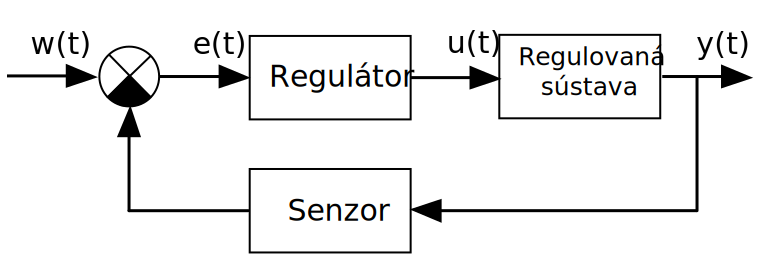
\includegraphics[width=120mm]{obr/pid.png}
	\caption{Schéma riadenia PID regulátorom.}\label{OBRAZOK 3.3}
\end{figure}

Skratka PID je zložená zo začiatočných písmen zložiek, z ktorých sa regulátor skladá. 

\begin{itemize}
	\item \textbf{P}- označuje tzv. proporcionálnu zložku. Akčný zásah \verb|u(t)|, je priamo úmerný veľkosti regulačnej odchýlky \verb|e(t)|. K$_p$ predstavuje proporcionálnu konštantu, ktorou násobíme regulačnú odchýlku na získanie požadovaného vstupu rov.\ref{rovnicajedna}. 
	\begin{align}
		\label{rovnicajedna}
		u(t)=K_p e(t)
	\end{align}
	Konštanta K$_p$ je veľmi dôležitou pri nastavovaní parametrov PID regulátora. Zvyšovaním hodnoty proporcionálnej zložky znižuje regulačnú odchýlku, avšak nikdy nedosiahneme úplne odstránenie trvalej regulačnej odchýlky. Zmenou proporcionálnej zložky vieme taktiež urýchliť, alebo spomaliť nábeh na požadovanú hodnotu. Pre malé hodnoty K$_p$ je nábeh pomalý, a regulačná odchýlka veľká. Pri zvyšovaní hodnoty K$_p$ sa zrýchľuje nábeh, no zároveň narastá nežiadúce kmitanie sústavy. Zvyšovanie hodnoty K$_p$ má svoj limit, za ktorým sa sústava dostáva za hranicu stability a ďalšia regulácia nie je možná. 
	
	\item \textbf{I}- predstavuje integračnú zložku. Integrálny riadiaci člen je priamo úmerný veľkosti chyby, ako aj dobe jej trvania. Pokiaľ má regulovaná veličina menšiu hodnotu ako je požadovaná, integrálna časť PID sa zväčšuje. Naopak pokiaľ je hodnota regulovanej veličiny väčšia ako požadovaná, integrálna časť PID klesá. Pri použití integračnej zložky PID regulátora, bude trvalá regulačná odchýlka nulová\cite{PIDcko}. Čím nižšia bude hodnota T$_i$ rov.\ref{rovnicatriapol}, tým rýchlejšie sa bude výstup približovať žiadanej hodnote, no zároveň však bude narastať kmitanie sústavy.   
	\begin{align}
		\label{rovnicadva}
		u(t)=K_i  \int_{0}^{t} e(\tau)d\tau  
	\end{align}
	\begin{align}
	\label{rovnicatriapol}
        T_i = \dfrac{K_p}{K_i}
    \end{align}
	
	\item \textbf{D}- reprezentuje derivačnú zložku, ktorá predpovedá správanie sa systému, pomocou derivácie regulačnej odchýlky v čase. Rýchlosť zmeny je následne prenásobená derivačnou konštantou K$_d$. Vstup je počítaný podľa rov.\ref{rovnicatri}. Zvyšovanie derivačnej zložky PID regulátora tlmí kmitanie sústavy. Ak však zvolíme derivačnú konštantu priveľkú, kmitanie začne znova narastať\cite{PIDcko}. V praxi sa derivačná zložka veľmi nepoužíva a využívaný je P alebo PI regulátor\cite{1453566}. 
	\begin{align}
		\label{rovnicatri}
		u(t)=K_d  \dfrac{de(t)}{dt}
	\end{align}

\end{itemize}

Pre lepšie chápanie je v tab.\ref{PIDvplyv}\cite{pidcontrol} zhrnutý vplyv jednotlivých zložiek PID, na odozvu systému v uzatvorenej slučke a to pri zvyšovaní hodnoty K$_p$, K$_i$ a K$_d$\footnote[10]{Tabuľka slúži len ako pomôcka pre hrubé ladenia. Jednotlivé zložky PID regulátora, ako aj ich vplyv na sústavu, sú v realite previazané.}. 

\begin{table}[!tbh]
	\begin{tabular}{|c|c|c|c|c|c|}
		\hline
		& Regulačná odchýlka & Rýchlosť ustálenia & Prekmit & Rýchlosť odozvy & Stabilita \\ \hline
		K$_p$                    & znižuje            & malý vplyv         & zvyšuje      & zvyšuje         & znižuje           \\ \hline
		K$_i$                    & znižuje            & znižuje            & zvyšuje      & zvyšuje         & znižuje           \\ \hline
		K$_d$                    & malý vplyv         & zvyšuje            & znižuje      & znižuje         & zvyšuje           \\ \hline
	\end{tabular}
	\caption{Odozva systému na zmenu konštánt.}
	\label{PIDvplyv}
\end{table}

Spojením jednotlivých samostatných zložiek, získame kompletný vzťah pre PID regulátor rov.\ref{rovnicastr}.
\begin{align}
	\label{rovnicastr}
	u(t)=K_p e(t) + K_i  \int_{0}^{t} e(\tau)d\tau + K_d  \dfrac{de(t)}{dt}
\end{align}

\begin{align}
	\label{rovnicapat}
	u(t)=K_p \left(e(t) + \dfrac{1}{T_i}  \int_{0}^{t} e(\tau)d\tau + T_d  \dfrac{de(t)}{dt}\right)
\end{align}
Rovnica \ref{rovnicastr} predstavuje jeden z možných zápisov vzťahu pre PID regulátor. V praxi sa často využíva tvar rov.\ref{rovnicapat}, z dôvodu lepšej interpretácie parametrov, ktoré rovnicu tvoria. T$_i$ predstavuje integračnú a T$_d$ derivačnú časovú konštantu, pričom ich vzťah s konštantami K$_i$ a K$_d$ je v tvare T$_i$ = (K$_p$/K$_i$) a T$_d$ = (K$_d$/K$_p$). Jednotlivé zložky v zátvorke tvoria novú a samostatnú regulačnú odchýlku, ktorá je ešte násobená konštantou K$_p$. Derivačná zložka predpovedá hodnotu regulačnej odchýlky T$_d$ sekúnd(vzoriek) do budúcnosti a integračná zložka sa snaží korigovať súčet hodnoty regulačných odchýlok do T$_i$ sekúnd(vzoriek)\cite{pidcontrol}.

Predchádzajúce rovnice PID regulátorov fungujú pri spojitých procesoch. Avšak pri implementácii PID pomocou číslicových regulátorov, musíme rovnicu transformovať do jej diskrétnej podoby rov.\ref{diskretna}.

\begin{align}
	\label{diskretna}
	u(kT)=K_p \left(e(kT) + \dfrac{T}{T_i} \sum_{i=0}^{k}  e(iT) + \dfrac{T_d}{T} \left[e(kT)-e \left[(k - 1)T\right] \right] \right)
\end{align}

Diskrétna forma PID regulátora je využívaná z toho dôvodu že Arduino resp. počítače nie sú schopné nepretržito zaznamenávať merané hodnoty. Dáta sú preto spracovávané v diskrétnych časových intervaloch \verb|kT|, ktorým hovoríme vzorky. Proces získavania takýchto vzoriek v istej pravidelnom frekvencii, nazývame vzorkovanie. 

Vzorkovanie môže mať rýchlosť niekoľko minút, pri pomaly sa meniacich procesoch, až po mikrosekundy pri procesoch dynamických. Rovnicu v tvare \ref{diskretna} využíva na implementáciu PID regulátora knižnica AutomationShield. 

\section{Programy v uzatvorenej slučke, so spätnou väzbou}
\subsection{Arduino IDE}
\label{sospatnou}
\label{Arduino IDE PID}

V tomto príklade využívame na riadenie PID regulátora, vopred pripravenú knižnicu \verb|PIDAbs|, ktorá je volaná z knižnice \verb|AeroShield|. Za účelom vzorkovania, využívame knižnicu \verb|Sampling|, ktorú načítame do príkladu príkazom \code{#include <Sampling.h>}. Pri voľbe referenčnej trajektórie máme na výber z dvoch možností. Prvou je voľba manuálnej trajektórie, ktorej referenčnú hodnotu nastavujeme pomocou potenciometra na shielde. Druhou voľbou je automatická trajektória, ktorá má vopred naprogramované referenčné hodnoty. Možnosti zadávania trajektórie meníme zmenou hodnoty premennej \verb|MANUAL| z 0 na 1 v príkaze \code{#define MANUAL 0}. Parametre regulátora K$_p$, T$_i$ a T$_d$ slúžia ako symbolické parametre, pre lepší prehľad. Ich hodnotu zapisujeme do PID knižnice pomocou metódy \code{PIDAbs.setKp(KP)}. Vzorkovacia perióda \verb|Ts| je nastavená na hodnotu troch milisekúnd. Perióda vzorkovania je priradená riadiacemu algoritmu PID, ako aj knižnici na vzorkovanie. 

\begin{lstlisting}[caption={Načítanie knižníc a premenných do programu.},captionpos=b]
	#define KP 1.7          // PID Kp konstanta
	#define TI 3.8          // PID Ti konstanta
	#define TD 0.25         // PID Td konstanta
	
	float startAngle=0;     //  Premenna pre nulovy uhol kyvadla
	float lastAngle=0;      //  Premenna pre mapovanie uhlu kyvadla
	float pendulumAngle;    //  Realna hodnota uhlu kyvadla
	
	unsigned long Ts = 3;   // Vzorkovacia perioda 
	unsigned long k = 0;    // Index vzorky 
	bool nextStep = false;  // Povolenie kroku vzorky 
	bool realTimeViolation = false;     // Premenna pri poruseni vzorkovania
	
	int i=i;                // Index referencnej hodnoty 
	int T=1000;             // Dlzka sekcie dana poctom vzoriek 
	float R[]={45.0,23.0,75.0,32.0,58.0,10.0,35.0,
		19.0,9.0,43.0,23.0,65.0,15.0,80.0};  // Referencna trajektoria kyvadla
	float r = 0.0;          // Referencia (Uhol ktory chceme dosiahnut)
	float y = 0.0;          // Vystup (Realny uhol kyvadla)
	float u = 0.0;          // Vstup (Vykon motora)
\end{lstlisting}

V organizačnej funkcii setup sa nastaví rýchlosť sériovej komunikácie, spolu s inicializáciou a kalibráciou AeroShieldu. Zároveň sa nastavia hodnoty PID 
regulátora, ako aj rýchlosť vzorkovania.  

\begin{lstlisting}[caption={Organzačná funkcia setup.},captionpos=b]
	void setup() {   
		Serial.begin(250000);      //  Zaciatok seriovej komunikacie
		AeroShield.begin();   //  Inicializacia 
		startAngle = AeroShield.calibration(AeroShield.getRawAngle());        // Kalibracia
		lastAngle=startAngle+1024;       // Vypocet uhlu pre mapovanie 
		Sampling.period(Ts*1000);              // Vzorkovacia perioda 
		PIDAbs.setTs(Sampling.samplingPeriod); // Vzorkovacia perioda
		Sampling.interrupt(stepEnable);  				   // Nasatavenie nazvu funkcie stepEnable, v kniznici sampling 
	}
\end{lstlisting}

Funkcia \verb|stepEnable()| je volaná z knižnice sampling, v intervale zadanom na začiatku programu, ako vzorkovacia perióda. Slúži na kontrolu postupnosti vzoriek a povolenie spustenia nasledujúcej vzorky. Táto funkcia je volaná vždy len na začiatku jednotlivých vzoriek. Pokiaľ je teda v trvaní jednej vzorky spustená viacero krát, vieme povedať že nastala chyba vzorkovania. Pri takejto chybe sa vypne motor a pomocou príkazu \code{while(1)}, je ukončené vykonávanie programu. 

Pokiaľ nedošlo ku chybe vzorkovania, funkcia povolí vykonanie nasledujúcej vzorky, zmenou hodnoty premennej \verb|nextStep|, na hodnotu $"$true$"$ teda 1. 

\begin{lstlisting}[caption={Funkcia stepEnable().},captionpos=b]
	void stepEnable() {                          
		if(nextStep == true) {        // Pokial predosla vzorka stale trva
			realTimeViolation = true; // Nastala chyba vzorkovania
			Serial.println("Real-time samples violated."); 			// Vypis chybovu hlasku
			analogWrite(5,0);         // Vypni motor 
			while(1);                 // Ukonci vykonavanie programu
		}
		nextStep = true;              // Povol nasledujucu vzorku
	}
\end{lstlisting}

V organizačnej funkcii \code{loop()}, je ako prvá, kontrolovaná podmienka \code{if(pendulumAngle>120)}. Táto kontrola slúži ako ochranný mechanizmus, pred pretočením kyvadla o príliš veľký uhol. Ďalej je v rámci vzorkovania volaná funkcia \verb|step()|. V if podmienke je testovaná premenná nextStep. Pokiaľ táto premenná nadobudne hodnotu "true", teda 1, podmienka sa splní a vykoná sa funkcia \verb|step()|, za ktorou sa premennej nextStep priradí hodnota "false", teda 0.

\begin{lstlisting}[caption={Organzačná funkcia loop.},captionpos=b]
	void loop() {
		if(pendulumAngle>120){		// Bezpecnostna podmienka kyvadla 
			AeroShield.actuatorWrite(0); // Pokial je uhol vacsi ako 120
			while(1);		// stupnov, motor sa vypne
		} 
		if (nextStep) {         // Pokial nextStep == 1
			step();             // Spusti funciu step()
			nextStep = false;   // Vynuluj premennu 
		}
	}
\end{lstlisting}

Funkcia \verb|step()| vykonáva samotné meranie, ovládanie a výpočty potrebné pri riadení systému pomocou PID regulátora. Na začiatku funkcie sa zvolí buď manuálna, alebo automatická trajektória. Pri automatickej dráhe je dôležité, vedieť kedy bol dosiahnutý koniec predprogramovanej trajektórie. Táto kontrola je vykonávaná pomocou porovnávania veľkostí premennej \verb|i|, ktorá zaznamenáva počet vykonaných sekcií trajektórie, oproti veľkosti pola \verb|R[]|, v ktorom sú zapísané hodnoty jednotlivých sekcií. Príkaz \code{sizeof(R)/sizeof(R[0])}, vráti počet prvkov pola \verb|R[]|. Zároveň sa kontroluje dĺžka chodu sekcie. Pokiaľ výraz \verb|k % (T*i)|, dosiahne hodnotu 0, nastaví sa ako trajektória nasledujúca sekcia. 

Následne je mapovaný uhol kyvadla na percentuálnu hodnotu od 0\% do 100\%, ktorá je uložená ako premenná \verb|y|. Veľkosť regulačnej odchýlky, obmedzenie integračného nasýtenia\footnote[11]{K nasýteniu integračnej zložky dochádza, v prípade že akčný člen nie je schopný dosiahnuť požadovanú referenčnú
	hodnotu. V takom prípade začne hodnota integračná zložka nekontrolovateľne stúpať.}(angl. anti-windup), ako aj hodnotu saturácie systému\footnote[12]{Ak sa ktorákoľvek so zložiek PID regulátora dostane do oblasti nasýtenia, ďalšia zmena tejto zložky nevyvolá žiadnu odozvu.}, zadávame do algoritmu na výpočet akčného zásahu v tvare \verb|PIDAbs.compute(r-y,minSaturacia,maxSaturacia|
\verb|,antiWindupMin,antiWindupMax);|. 


\begin{lstlisting}[caption={Funkcia step().},captionpos=b]
	void step() {            
		#if MANUAL    // Pokial je zvolena manualna trajektoria 
		r = AeroShield.referenceRead();     // Referencna hodnota z potenciometra
		#else         
		if(i>(sizeof(R)/sizeof(R[0]))) {    // Pokial automaticka trajektoria skoncila
			analogWrite(5,0);           // Vypni motor
			while(1);                   // Zastav program
		} else if (k % (T*i) == 0) {  // Pokial je dosiahnuty koniec       sekcie trajektorie
			r = R[i];        // Postup na dalsiu sekciu
			i++;             // Pripocitaj postup o jednu sekciu 
		}
		#endif
		
		y= AutomationShield.mapFloat(AeroShield.getRawAngle(),startangle,lastangle,0.00,100.00);
		// Mapovanie uhlu kyvadla na percenta 
		u = PIDAbs.compute(r-y,0,100,0,100);  // Vypocet PID 
		AeroShield.actuatorWrite(u);          // Aktuator
		
		Serial.print(r);           // Referencna hodnota 
		Serial.print(", ");
		Serial.print(y);           // Vystup 
		Serial.print(", ");
		Serial.println(u);         // Akcny zasah 
		k++;                       // Pocitadlo vzoriek 
	}
\end{lstlisting}

\subsubsection{Výstupy}

Všetky výstupy z API Arduino IDE, boli zaznamenávané programom CoolTerm a následne vykreslené do grafov v prostredí MATLAB. 

Na obr.\ref{OBRAZOK 2.5.1}, vidíme reakciu systému na skokovú zmenu z nulovej referenčnej hodnoty na hodnotu maximálnu, teda 100\%. Pomocou sledovania odozvy systému vieme lepšie nastaviť parametre PID regulátora. Systém nadobudne 1\% regulačnú odchýlku v priebehu 500 vzoriek, čo znamená čas približne jeden a pol sekundy. 

\begin{figure}[!tbh]
	\centering
	\includegraphics[width=120mm]{obr/SkokovaZmena.png}
	\caption{Reakcia systému na skokovú zmenu referenčnej hodnoty- Arduino IDE.}\label{OBRAZOK 2.5.1}
\end{figure}

Manuálna trajektória obr.\ref{OBRAZOK 2.5.3}, má oproti automatickej trajektórii obr.\ref{OBRAZOK 2.5.2}, väčšie rozdiely v hodnote akčného zásahu. Je to spôsobené kontinuálnou zmenou referenčnej hodnoty, ako aj miernym šumom signálu z potenciometra. V rámci obr.\ref{OBRAZOK 2.5.3} si ešte môžeme všimnúť časť medzi vzorkami 5000-6000. Ide o manuálne zavedenie chyby, pomocou buchnutia do kyvadla. Systém na takúto zmenu reaguje zmenou akčného zásahu a regulačnú odchýlku menšiu ako 2\%, nadobúda v priebehu jednej sekundy. 

\begin{figure}[!tbh]
	\centering
	\includegraphics[width=150mm]{obr/Auto3.png}
	\caption{Automatická trajektória.}\label{OBRAZOK 2.5.2}
\end{figure}

\begin{figure}[!tbh]
	\centering
	\includegraphics[width=150mm]{obr/potentio.png}
	\caption{Manuálna trajektória.}\label{OBRAZOK 2.5.3}
\end{figure}


\subsection{MATLAB}
\label{MATLABPID}

Príklad na ukážku fungovania PID regulátora bol taktiež vytvorený v prostredí MATLAB a simulink. V prípade MATLABU využívame, na výpočet akčného zásahu, knižnicu PID.m, ktorá bola taktiež vytvorená v rámci programu AutomationShield. Na nastavenie parametrov PID slúži príkaz \code{PID.setParameters(Kp, Ti, Td, Ts)}. 

Na vzorkovanie využívame funkcie \verb|TIC a TOC |, ktoré merajú prejdený čas. Funkcia TIC zaznamenáva aktuálny čas a funkcia TOC používa zaznamenanú hodnotu na výpočet uplynulého času. Ak je splnená podmienka \code{if (toc>=Ts*k)}, povolí sa posun na nasledujúcu vzorku, pričom premenná \verb*|k|, udáva počet vykonaných vzoriek. Dáta sú postupne zapisované do poľa \code{ PIDresponse(k,:)=[r y u]}, a toto pole je vykresľované pomocou funkcie \code{plotLive(PIDresponse(k,:))}. Na konci sú všetky dáta uložené, a teda sú prístupné aj po ukončený programu. Kompletný zdrojový kód sa nachádza v prílohe \ref{AeroShieldPID.m}.

Regulácia PID v prostredí MATLAB potrebuje pre svoje fungovanie pomerne vysoký výpočtový výkon počítača, pretože výpočty prebiehajú na zariadení, s ktorým je Arduino prepojené. Na zariadení \cite{Notebook} v ktorom boli písané všetky didaktické príklady dosahujeme rýchlosť maximálne piatich vzoriek za sekundu tj. Ts=0.2s. Pri pomalšom vzorkovaní musíme spomaliť aj rýchlosť reakcie PID regulátora (napr. znížením proporcionálnej zložky), inak regulácia prestane byť možná. Výpočtová náročnosť sa dá znížiť, zamedzením vykresľovania grafu, alebo odstránením možnosti ukladania zaznamenaných dát. 

\begin{figure}[!tbh]
	\centering
	\includegraphics[width=90mm]{obr/jednotkovyskoskMAt.png}
	\caption{Reakcia systému na skokovú zmenu referenčnej hodnoty- MATLAB.}\label{OBRAZOK 2.6.1}
\end{figure}

\subsubsection{Výstupy}

Všetky výstupy z príkladu \ref{MATLABPID}, majú priamu funkciu vykresľovania grafov spolu s legendou výstupov. Tieto grafy majú taktiež definovaný rozsah zobrazovaných hodnôt na oboch osiach, ako aj pomenovania týchto osí. Na Obr. \ref{OBRAZOK 2.6.1} vidíme reakciu systému na jednotkový skok. Obrázok \ref{OBRAZOK 2.6.2} zobrazuje automatickú trajektóriu referenčnej hodnoty a Obr. \ref{OBRAZOK 2.6.3} trajektóriu manuálnu. 

Pri manuálnej trajektórii bola trikrát vnesená veľká chyba a to pomocou úderu do kyvadla. Ako je vidieť z grafu \ref{OBRAZOK 2.6.3}, ustálenie systému prebieha oveľa pomalšie ako v príklade \ref{Arduino IDE PID}. Oscilácia je pomerne vysoká a pretrváva po dobu cca 35 vzoriek, čo predstavuje približne 7 sekúnd. Táto skutočnosť je spôsobená pomalšou reakciou PID regulátora, na veľkú regulačnú odchýlku. Dlhší čas potrebný na ustálenie kyvadla je spôsobený predovšetkým pomalším vzorkovaním. 

\begin{figure}[!tbh]
	\centering
	\includegraphics[width=125mm]{obr/PIDautomaMat.png}
	\caption{Automatická trajektória.}\label{OBRAZOK 2.6.2}
\end{figure}
\begin{figure}[!tbh]
	\centering
	\includegraphics[width=125mm]{obr/pidmanualbuchh.png}
	\caption{Manuálna trajektória.}\label{OBRAZOK 2.6.3}
\end{figure}

\newpage 
\subsection{Simulink}

Vzhľadovo pôsobí príklad PID riadenia v API Simulink jednoducho a elegantne. Predpripravené bloky z knižnice AeroLibrary stačí v príklade pospájať podľa potreby a následne zvoliť vhodné parametre v maskách blokov. Prepájanie blokov slúži na spájanie vstupov s výstupmi, alebo na matematické operácie s premennými. Regulovanú sústavu v tomto príklade predstavuje blok \verb|AeroShield|, do ktorého vstupuje z bloku \verb|Reference read| percentuálna hodnota referenčnej trajektórie. Z bloku \verb|AeroShield| získavame ako výstup uhol kyvadla, ktorý využívame na výpočet regulačnej odchýlky.  

Blok \verb|Discrete PID Controller| predstavuje riadiaci systém PID regulátora. Hodnoty jednotlivých zložiek regulátora sú: P=0.011, I=200, D=8. Matematická reprezentácia výpočtového algoritmu ideálneho PID regulátora, je v tvare Rov. \ref{PIDSimulink}:

\begin{equation}\label{PIDSimulink}
	P\left(1+I*T_s\dfrac{1}{z-1}+D*\dfrac{1}{T_s}\dfrac{z-1}{z}\right)
\end{equation}


\begin{figure}[!tbh]
	\centering
	\includegraphics[width=125mm]{obr/SimulinkPID.png}
	\caption{Ukážka riadenia systému pomocou PID regulátora v API Simulink.}\label{OBRAZOK 2.6.10}
\end{figure}

\subsubsection{Výstupy}

\begin{figure}[!tbh]
	\centering
	\includegraphics[width=100mm]{obr/SimSkok.png}
	\caption{Reakcia systému na skokovú zmenu referenčnej hodnoty- Simulink.}\label{OBRAZOK 2.6.11}
\end{figure}

\begin{figure}[!tbh]
	\centering
	\includegraphics[width=125mm]{obr/SimulinkManualBuch.png}
	\caption{Manuálna trajektória.}\label{OBRAZOK 2.6.12}
\end{figure}
\chapter{Záver}

Príkladmi z kapitoly \ref{Didaktické príklady} a \ref{PIDPID}, sme potvrdili funkčnosť AeroShieldu v API Arduino IDE, MATLAB a Simulink. AeroShield je teda použiteľný ako didaktická pomôcka a to aj napriek niektorým nedostatkom na softvérovom, ako aj hardvérovom rozhraní. 

Na AeroShielde je zaznamenávaný prúd, ktorý odoberá akčný člen sústavy. Toto meranie je pri malých zmenách prúdu pomerne nepresné a to z dôvodu ovládania motora PWM signálom. V budúcej verzii AeroShieldu môže byť použitý iný druh napájania motora, čo by malo za následok aj vylepšenie presnosti merania prúdu. Takto nameraný prúd by sa dal následne využívať na presnejšie riadenie výkonu motora, alebo na implementáciu PID regulácie na základe prúdu a nie uhlu kyvadla. 

Ďalším problémom pri PID regulácii AeroShieldu, je jeho zložité a dlhotrvajúce nastavenie parametrov. Pri príklade \ref{MATLABPID} na strane \pageref{MATLABPID}, bolo nastavenie parametrov najzložitejšie a strávil som pri ňom niekoľko desiatok hodín. Problémom bolo pomalšie vzorkovanie a teda aj malá zmena parametrov, spôsobila veľké zmeny na výstupe. 

Ďalším z problémov bolo priame prepojenie motora so Shieldom. V prípade nechceného pretočenia ramena kyvadla, sa napájacie káble zapletú na rameno a to spôsobý zamedzenie ďalšieho otáčania. Všetky didaktické príklady síce majú implementovanú softvérovú ochranu proti takémuto pretočeniu, avšak táto nie je 100\% účinná. 
Tento problém by vyriešila realizácia napájania pomocou konektora so zbernými krúžkami, avšak takýto konektor stojí v priemere 15\euro  a teda jeho aplikácia v nízko nákladovej učebnej pomôcke je otázna. Zároveň pomocou magnetu uloženého na konci kyvadla meriame jeho uhol. Použitý konektor by preto musel mať stredovú časť s možnosťou pripevnenia magnetu, alebo by sa uhol kyvadla musel merať iným spôsobom. 

Medzi vylepšenia nasledujúceho modelu AeroShieldu môžeme zaradiť úplnú zmenu podporného systému kyvadla. Uchytenie pomocou dvoch otočených \verb|V| konštrukcií, prepojených priečkou, by umožňovalo meranie natočenia na jednej strane priečky a druhou stranou by bolo realizované napájanie motora. Zaujímavým experimentom by bola možnosť hardvérovej zmeny smeru otáčania motora, pomocou prepínača. Pokiaľ by bola rýchlosť zmeny otáčania dostatočne rýchla (rádovo niekoľko desiatok milisekúnd), dal by sa realizovať príklad otočeného kyvadla, kedy je rameno kyvadla držané pomocou regulátora vo vzpriamenej polohe.   

Medzi dalšie vylepšenia pre budúcu prácu s AeroShieldom, môžeme zaradiť reguláciu pomocou iného algoritmu ako bol PID. Medzi ne môžeme zaradiť modelové prediktívne riadenie (MPC), Lineárno-kvadratické riadenie (LQ), Lineárne riadenie s premenlivým parametrom (LPV)... Pomocou týchto algoritmov by sme mohli dosiahnuť lepšie vlastnosti systému a tým pádom presnejšie riadenie. 

Všetky chyby a nedokonalosti dizajnu, ako aj neschopnost dokonalého nastavenia uhlu kyvadla pri PID regulácii,
neznemožňujú kvalitnú výuku s použitím AeroShieldu. Sú to skôr nápady a možnosti vylepšenia, ktoré môžu byť v budúcnosti na AeroShield implementované.

%%%%%%% Koniec %%%%%%%%

\bibliographystyle{unsrt}
\addcontentsline{toc}{chapter}{Literat\'{u}ra}
\bibliography{bibliog}
\backmatter
\pagenumbering{roman}\setcounter{page}{4}
\cleardoublepage
% \phantomsection
\addcontentsline{toc}{chapter}{Arduino IDE}
\addcontentsline{toc}{section}{Zdrojový kód AeroShield.h}
\LARGE\bf{Zdrojový kód súboru AeroShield.h}
\label{AeroShield.h}
\vspace{1cm}
\begin{lstlisting}[numbers=left,basicstyle=\scriptsize,caption={Zdrojový kód súboru AeroShield.h.},captionpos=b,]	
	#ifndef AEROSHIELD_H			 
	#define AEROSHIELD_H	
	
	#include "AutomationShield.h" 
	#include <Wire.h>              
	#include <Arduino.h>			 
	#define AERO_RPIN A3        
	#define VOLTAGE_SENSOR_PIN A2   
	#define AERO_UPIN 5   
	
	class AeroShield{		    	               
		public:
		AeroShield(void);
		void begin(void);                                       
		void actuatorWrite(float PotPercent);          
		float calibration(word RawAngle);          
		float convertRawAngleToDegrees(word newAngle);  
		float referenceRead(void);
		float currentMeasure(void);
		int detectMagnet();	
		int getMagnetStrength();
		word getRawAngle();
		
		private:
		int ang;                                        
		float startangle;                              
		float referenceValue;               
		float referencePercent;              
		float correction1= 4.1220;			
		float correction2= 0.33;			
		int repeatTimes= 100;				
		float voltageReference= 5.0;		
		float ShuntRes= 0.1;				
		float current;						
		float voltageValue;				
		int _ams5600_Address = 0x36;	
		int _stat = 0x0b;				
		int _raw_ang_hi = 0x0c;		
		int _raw_ang_lo = 0x0d;		
		int readOneByte(int in_adr);	
		word readTwoBytes(int in_adr_hi, int in_adr_lo); 
	};
	#endif
\end{lstlisting}
\addcontentsline{toc}{section}{Zdrojový kód AeroShield.cpp}
\LARGE\bf{Zdrojový kód súboru AeroShield.cpp}
\label{AeroShield.cpp}
\vspace{1cm}
\begin{lstlisting}[numbers=left,basicstyle=\tiny,caption={Zdrojový kód súboru AeroShield.cpp.},captionpos=b]	
	#include "AeroShield.h"     
	
	float AeroShield::begin(bool isDetected){   
		pinMode(AERO_UPIN,OUTPUT);  		   
		#ifdef ARDUINO_ARCH_AVR      
		Wire.begin();                            
		#elif ARDUINO_ARCH_SAM                            
		Wire1.begin();                
		#elif ARDUINO_ARCH_SAMD         
		Wire.begin();                            
		#endif
		
		if(isDetected == 0 ){                
			while(1){                                    
				if(isDetected == 1 ){                          
					AutomationShield.serialPrint("Magnet detected \n");
					break;
				}
				else{                                                 
					AutomationShield.serialPrint("Can not detect magnet \n"); 
				}
			}
		}       
	} 
	
	float AeroShield::convertRawAngleToDegrees(word newAngle) {
		float retVal = newAngle * 0.087;      
		ang = retVal;                               
		return ang;                  
	}
	
	float AeroShield::calibration(word RawAngle) {      
		AutomationShield.serialPrint("Calibration running...\n");  
		startangle=0;                                
		analogWrite(AERO_UPIN,50);              
		delay(250);                              
		analogWrite(AERO_UPIN,0);              
		delay(4000);    
		
		startangle = RawAngle;                                 
		analogWrite(AERO_UPIN,0);                     
		for(int i=0;i<3;i++){                  
			analogWrite(AERO_UPIN,1);                 
			delay(200);                           
			analogWrite(AERO_UPIN,0);                                
			delay(200);                                     
		}
		AutomationShield.serialPrint("Calibration done");
		return startangle;                                         
	}
	
	float AeroShield::referenceRead(void) {                                                
		referencePercent = AutomationShield.mapFloat(analogRead(AERO_RPIN), 0.0, 1024.0, 0.0, 100.0);   
		return referencePercent;                                     
	}
	
	void AeroShield::actuatorWrite(float PotPercent) {       
		float mappedValue = AutomationShield.mapFloat(PotPercent, 0.0, 100.0, 0.0, 255.0);  
		mappedValue = AutomationShield.constrainFloat(mappedValue, 0.0, 255.0);
		analogWrite(AERO_UPIN, (int)mappedValue);    
	}
	
	float AeroShield::currentMeasure(void){       
		for(int i=0 ; i<repeatTimes ; i++){                                            
			voltageValue= analogRead(VOLTAGE_SENSOR_PIN);                                       
			voltageValue= (voltageValue * voltageReference) / 1024;                             
			current= current + correction1-(voltageValue / (10 * ShuntRes));     
		}                                                              
		float currentMean= current/repeatTimes;             
		currentMean= currentMean-correction2;              
		if(currentMean < 0.000){                           
			currentMean= 0.000;                             
		}
		current= 0;               
		voltageValue= 0;         
		return currentMean;  
	}
	
	word AeroShield::getRawAngle()                                                           
	{
		return readTwoBytes(_raw_ang_hi, _raw_ang_lo);                                         
	}
	
	int AeroShield::detectMagnet()                                                         
	{
		int magStatus;                                                                   
		int retVal = 0;                                                                      
		magStatus = readOneByte(_stat);                                                                  
		if (magStatus & 0x20)
		retVal = 1;
		return retVal;                                                               
	}
	
	int AeroShield::getMagnetStrength()           
	{
		int magStatus;                                 
		int retVal = 0;                             
		magStatus = readOneByte(_stat);               
		if (detectMagnet() == 1)                         
		{	retVal = 2;                               
			if (magStatus & 0x10)
			retVal = 1;                               
			else if (magStatus & 0x08)
			retVal = 3;                            
		} return retVal;                          
	}
	
	int AeroShield::readOneByte(int in_adr)       
	{
		int retVal = -1;
		Wire.beginTransmission(_ams5600_Address);     
		Wire.write(in_adr);                            
		Wire.endTransmission();                         
		Wire.requestFrom(_ams5600_Address, 1);          
		while (Wire.available() == 0);                   
		retVal = Wire.read();                         
		return retVal;                                   
	}
	
	word AeroShield::readTwoBytes(int in_adr_hi, int in_adr_lo)     
	{
		word retVal = -1;
		/* Read Low Byte */
		Wire.beginTransmission(_ams5600_Address);     
		Wire.write(in_adr_lo);                        
		Wire.endTransmission();                        
		Wire.requestFrom(_ams5600_Address, 1);          
		while (Wire.available() == 0);                  
		int low = Wire.read();                    
		
		/* Read High Byte */
		Wire.beginTransmission(_ams5600_Address);       
		Wire.write(in_adr_hi);                    
		Wire.endTransmission();                       
		Wire.requestFrom(_ams5600_Address, 1);        
		while (Wire.available() == 0);               
		word high = Wire.read();                    
		high = high << 8;                             
		retVal = high | low;
		return retVal;                                
	}	
\end{lstlisting}
\addcontentsline{toc}{section}{Zdrojový kód AeroShieldOpenLoop.ino}
\LARGE\bf{Zdrojový kód súboru AeroShieldOpenLoop.ino}
\label{AeroShieldOpenLoop.ino}
\vspace{1cm}
\begin{lstlisting}[numbers=left,basicstyle=\scriptsize,caption={Zdrojový kód súboru AeroShieldOpenLoop.ino.},captionpos=b]	
	#include "AeroShield.h" 
	
	float startAngle=0; 
	float lastAngle=0; 
	float pendulumAngle;  
	float referencePercent;  
	float CurrentMean; 
	
	void setup() {
		
		Serial.begin(115200);   
		AeroShield.begin(AeroShield.detectMagnet());
		startAngle = AeroShield.calibration(AeroShield.getRawAngle());
		lastAngle=startAngle+1024;  
	}
	
	void loop() {
		if(pendulumAngle>120){
			AeroShield.actuatorWrite(0);
			while(1);
		}
		
	pendulumAngle= AutomationShield.mapFloat(AeroShield.getRawAngle(),startAngle,lastAngle,0.00,90.00);  
	referencePercent= AeroShield.referenceRead(); 
	AeroShield.actuatorWrite(referencePercent);    
	CurrentMean= AeroShield.currentMeasure();

	Serial.print(pendulumAngle);  
	Serial.print(" ");
	Serial.print(referencePercent); 
	Serial.print(" ");
	Serial.println(CurrentMean);
	}
\end{lstlisting}
\addcontentsline{toc}{section}{Zdrojový kód AeroShieldPID.ino}
\include{AeroShieldPID.ino}
\addcontentsline{toc}{chapter}{MATLAB}
\addcontentsline{toc}{section}{Zdrojový kód AeroShield.m}
\LARGE\bf{Zdrojový kód súboru AeroShield.m}
\label{AeroShield.m}
\vspace{1cm}
\begin{lstlisting}[numbers=left,basicstyle=\scriptsize,caption={Zdrojový kód súboru AeroShield.m.},captionpos=b]	
	classdef AeroShield < handle
	
	properties
	arduino;
	as5600;
	end
	properties(Constant)
	AERO_UPIN = 'D5'; 
	AERO_RPIN = 'A3';
	VOLTAGE_SENSOR_PIN = 'A2';
	voltageReference = 5.0;
	ShuntRes = 0.1;
	correction1 = 4.1220;
	correction2 = 0.33;
	repeatTimes = 50;
	end
	
	methods
	function begin(AeroShieldObject) 
	AeroShieldObject.arduino = arduino();
	AeroShieldObject.as5600 = device(AeroShieldObject.arduino,'I2CAddress',0x36); 
	configurePin(AeroShieldObject.arduino,AeroShieldObject.AERO_UPIN, 'DigitalOutput') 
	disp('AeroShield initialized.') 
	end
	function startangle = calibration(AeroShieldObject)
	write(AeroShieldObject.as5600, 0x0c, 'uint8');
	write(AeroShieldObject.as5600, 0x0d, 'uint8');
	startangle = read(AeroShieldObject.as5600, 1, 'uint16');
	end
	function PWM = referenceRead(AeroShieldObject)
	PWM= readVoltage(AeroShieldObject.arduino, AeroShieldObject.AERO_RPIN);
	end
	function actuatorWrite(AeroShieldObject, PWM) 
	writePWMVoltage(AeroShieldObject.arduino, AeroShieldObject.AERO_UPIN, PWM);
	end
	function RAW = getRawAngle(AeroShieldObject)
	write(AeroShieldObject.as5600, 0x0c, 'uint8');
	write(AeroShieldObject.as5600, 0x0d, 'uint8');
	RAW = read(AeroShieldObject.as5600, 1, 'uint16');
	end
	function currentMean = getCurrent()
	for r = 1:repeatTimes
	voltageValue = readVoltage(AeroShieldObject.arduino, AeroShieldObject.VOLTAGE_SENSOR_PIN);
	voltageValue= (voltageValue * voltageReference) / 1024;
	Current= Current + correction1-(voltageValue / (10 * ShuntRes)); 
	end
	currentMean= Current/repeatTimes;
	currentMean= currentMean-correction2;
	if currentMean < 0.000 
	currentMean= 0.000; 
	end
	current= 0;  
	voltageValue=0;   
	end 
	end
	end
\end{lstlisting}
\addcontentsline{toc}{section}{Zdrojový kód AeroShieldOpenLoop.m}
\LARGE\bf{Zdrojový kód súboru AeroShieldOpenLoop.m}
\label{AeroShieldOpenLoop.m}
\vspace{1cm}
\begin{lstlisting}[numbers=left,basicstyle=\scriptsize,caption={Zdrojový kód súboru AeroShieldOpenLoop.m.},captionpos=b]	
	clear all;
	clear a;
	clc 
	
	AeroShield=AeroShield;
	AeroShield.begin();
	startangle= AeroShield.calibration(); 
	lastangle=startangle+2048;
	
	time = 0;
	count = 0;
	angle = 0;
	potentiometer = 0;
	
	yyaxis right  
	plotGraph = plot(time,angle,'-r' )
	ylabel('Angle (degree)','FontSize',15);
	xlabel('Time (s)','FontSize',15); 
	hold on  
	
	yyaxis left 
	plotGraph1 = plot(time,potentiometer,'-b')
	title('Pendulum plot','FontSize',15);
	ylabel('Percent','FontSize',15)  
	legend('Potentiometer value','Pendulum angle')
	grid('on');
	
	tic    
	
	while ishandle(plotGraph)  
	pwm = AeroShield.referenceRead();
	AeroShield.actuatorWrite(pwm);
	
	RAW= AeroShield.getRawAngle();  
	angle_ = mapped(RAW, startangle, lastangle, 0, 180);
	count = count + 1;  
	time(count) = toc;      
	angle(count) = angle_(1);   
	percenta= mapped(pwm, 0.0, 5.0, 0.0, 100.0); 
	potentiometer(count) = percenta(1);          
	set(plotGraph,'XData',time,'YData',angle);   
	set(plotGraph1,'XData',time,'YData',potentiometer);
	axis([time(count)-5 time(count) 0 100]);  
	
	if (angle_ > 110)                         
	AeroShield.actuatorWrite(0.0);    
	disp('Angle of pendulum too high. AeroShield is turned off')
	break                              
	end
	end             
	
	clear AeroShield.arduino;
\end{lstlisting}
\addcontentsline{toc}{section}{Zdrojový kód AeroShielPID.m}
\include{ZdrojovyAeroShielPID.m}
\addcontentsline{toc}{chapter}{Simulink}
\end{document}
